\chapter{\textit{Pan troglodytes verus}}
\label{ch:chimp}

\begin{figure}[h!]
  \centering
    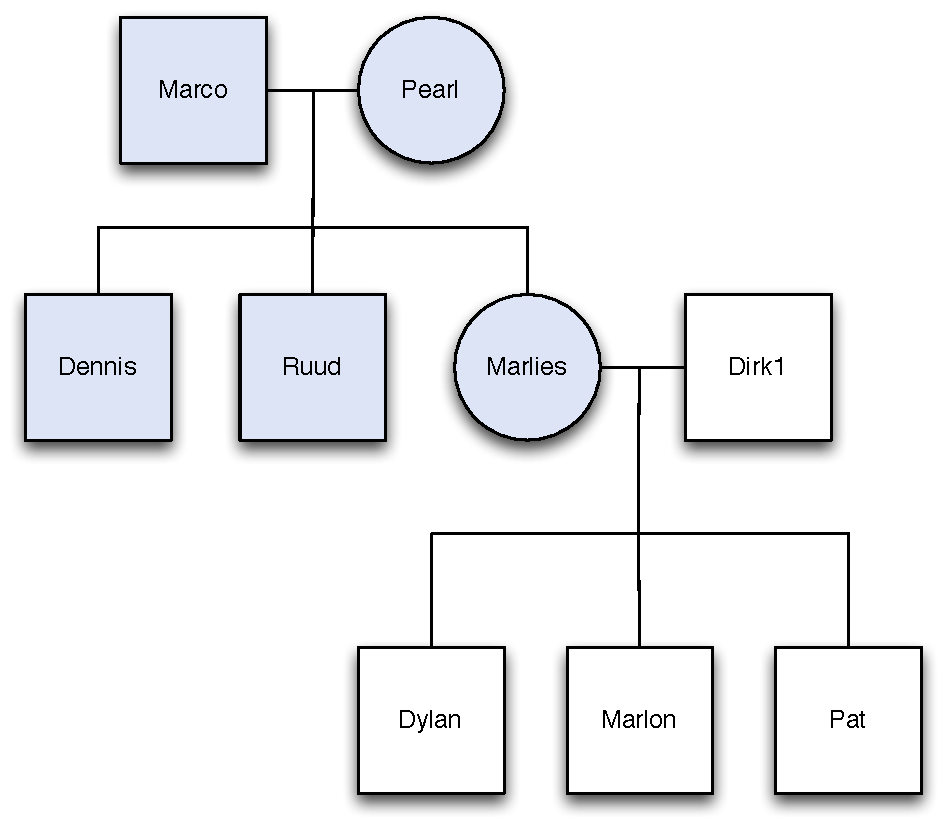
\includegraphics[width=0.7\textwidth]{pedigree}
  \caption{The three-generation chimpanzee pedigree.  The highlighted quintet is discussed in this chapter.}
  \label{fig:pedigree}
\end{figure}

Finally, we present our work on a second dataset: a quintet taken from a three-generation, nine member pedigree of West African chimpanzees (\textit{Pan troglodytes verus}).  The processed samples are highlighted in Figure \ref{fig:pedigree}.  Venn {et al.} have previously examined this pedigree using reference-based methods for \textit{de novo} variation discovery, reporting a substantial paternal age effect to the overall mutation rate\cite{Venn:2014ep}.

In many ways, the chimpanzee quartet is a more challenging dataset to process than the \textit{falciparum} crosses.  First, the genome is roughly two orders of magnitude larger; \textit{Plasmodium falciparum} is approximately $23$ Mbp, while \textit{Pan troglodytes} is $3,300$ Mbp ($3.3$ Gbp).  Second, the genome is diploid rather than haploid, an additional challenge during variant detection as now our software must contend with the presence of heterozygotes.  Third, we do not have draft-quality parental assemblies, and owing to the genome size, it is prohibitively expensive to generate such data as we did in the previous chapter.  We will be forced to rely solely on the Illumina data for the parents and children.  Fourth, the chimpanzee reference genome is reported to be of lesser quality than the \textit{falciparum} reference, misassemblies in which can contribute to false positive variant calls\cite{Mallick:2009go}.  The chimpanzee assembly process employed a whole-genome shotgun sequencing approach yielding $5x$ coverage and $37,846$ supercontigs that were aligned to the human reference build to reconstruct the autosomes and sex chromosomes\cite{ChimpanzeeSequencingandAnalysisConsortium:2005fa}.  The \textit{falciparum} employed a whole-chromosome shotgun approach yielding approximately $14x$ coverage per chromosome.  With myriad errors in the chimpanzee reference sequence, a method unbiased towards the reference sequence should prove quite useful.  Finally, the coverage is substantially lower: $57x$ on average for the founders, $28x$ on average for the children, or one-half and one-third the coverage we had for samples in the previous chapter.

For precisely these reasons, the chimpanzee dataset is an important test-bed for our \textit{de novo} mutation calling software.  It permits a demonstration of our capacity to process much larger genomes than the \textit{falciparum} parasite.  Moreover, the problematic chimpanzee reference sequence and infeasibility of generating draft reference assemblies for the parents or children allow us to demonstrate the value of an approach that can leverage both, but requires neither.

\section{Data processing}

\subsection{Initial data}

\begin{table}[]
\centering
\caption{Summary of \textit{P. troglodytes} quintet data}
\label{tbl:pedstats}
\begin{tabular}{@{}llllll@{}}
\toprule
                                       & Marco           & Pearl           & Dennis         & Ruud            & Marlies         \\ \midrule
Platform                               & \multicolumn{5}{c}{Illumina HiSeq 2000}                                                \\
Read length (bp)                       & \multicolumn{5}{c}{$100$}                                                              \\
Fragment size (bp)                     & $369 \pm 23$    & $399 \pm 31$    & $377 \pm 24$   & $415 \pm 27$    & $383 \pm 28$    \\
Coverage                               & $60 \pm 10$     & $54 \pm 8$      & $35 \pm 6$     & $22 \pm 3$      & $29 \pm 5$      \\
Cleaning threshold                     & $10$            & $9$             & $8$            & $4$             & $6$             \\
Kmers                                  &                 &                 &                &                 &                 \\
\multicolumn{1}{r}{\textit{dirty}}     & $7.7e9$         & $9.0e9$         & $5.9e9$        & $4.4e9$         & $5.2e9$         \\
\multicolumn{1}{r}{\textit{clean}}     & $2.6e9$         & $2.7e9$         & $2.5e9$        & $2.7e9$         & $2.6e9$         \\
Novel kmers                            &                 &                 &                &                 &                 \\
\multicolumn{1}{r}{\textit{initial}}   & -               & -               &                & $348,374$       & $121,834$       \\
\multicolumn{1}{r}{\textit{confident}} & -               & -               &                & $1,474$         & $2,197$         \\
\multicolumn{1}{r}{\textit{trusted}}   & -               & -               &                & $600$           & $1,034$         \\ \bottomrule
\end{tabular}
\end{table}

We obtained the raw genomic sequencing data for the nine members of the pedigree.  For simplicity, we chose to focus our efforts on three children in the $F_1$ generation: Dennis, Ruud, and Marlies.  Their parents, Marco and Pearl, were sequenced to higher coverage.  This should give us greater confidence in our ability to distinguish novel kmers, kmers present in the child but absent from the parents, from those only absent from the parental genomes due to issues with sequencing.  The quintet is summarized in Table \ref{tbl:pedstats}.

\subsection{Sample processing}

Precisely as we did for the \textit{P. falciparum} samples in the previous chapter, we used the available Illumina data to construct the de Bruijn graph structures for each child with McCortex, using a kmer size of $47$ bp and discarding bases with a quality score less than $Q5$.  McCortex's automatic cleaning algorithm was applied to the dirty graph for each sample.  We did not apply the paired-end read threading and contig emission steps as contigs were not required for our analysis.

\subsection{Novel kmers}

We produced a list of novel kmers per child in the manner described in Chapter \ref{ch:methods}, selecting kmers present in the child but absent in the parents ("initial" in Table \ref{tbl:pedstats}), then applying coverage thresholds ("confident") and non-chimpanzee contamination checks ("trusted") to the resulting list\footnote{Examining the results of the contamination check, it is evident that some samples contain small numbers of kmers that BLAST identifies as coming from human (hundreds) or gorilla (dozens).  Given the evolutionary relationships between the three species, it is perhaps not unreasonable to allow these kmers into the analysis, as they may misattributed in the BLAST database.  Instead, we have opted to remain conservative and exclude these from consideration.}.

\section{\textit{De novo} mutations in the \textit{P. troglodytes} dataset}

\subsection{\textit{De novo} mutations in a single sample}
\subsection{\textit{De novo} mutations in all progeny}
\subsubsection{Mutational spectrum}
\subsubsection{Comparison to published calls}
